\section{Preparação dos modelos}
\label{sec:metodos-preparacao-modelos}

% Uma vez que temos um \textit{dataset} com atributos fonológicos processados, agora podemos prosseguir com a preparação das features e dos modelos para reconhecimentos dos sinais utilizando a abordagem proposta.


% Experimento
%   Preparação das features (asl-phono -> palavras)
%       Transformação das sequências no dataset: frames -> palavras
%       Justificativa??
%   Preparação dos modelos (Transformer, LSTM, GRU, etc) -- por modelo
%       Arquitetura + Parâmetros
%       lr scheduler, optimizer, loss function
%       Busca de parâmetros (dimensionar os modelos/parâmetros)

%FIXME: [cz] essa parte ficaria na metodologia se vc tirar a os datasets para uma nova secao

% SELEÇÃO DOS MODELOS -------------------------------------------

Tomando como referência a discussão introduzida na \autoref{sec:modelos-sequenciais}, adotaremos nos experimentos deste trabalho três das principais arquiteturas utilizadas em tarefas de \acrfull{nlp}: o \textit{Encoder-Decoder} em uma versão com \acrfull{lstm} e em outra com \acrfull{gru}, e também o \textit{Transformer}.

% Os parâmetros para treinamento dos modelos foram selecionados com base na discussão apresentada por \citeonline{goodfellow-2016-deep-learning}, a qual aborda de forma prática temas como definição de métricas, modelos de base, otimização de parâmetros, entre outros para tal finalidade.

Para estabelecer os parâmetros dessas arquiteturas, as estratégias de otimização e treinamento, bem como as métricas a serem utilizadas nos experimentos, nos fundamentamos pela discussão apresentada por \citeonline{goodfellow-2016-deep-learning}.
Dessa forma, o algoritmo de otimização será definido como o \acrfull{sgd} com \textit{momentum} de 0,9. Ele será combinado a uma estratégia de redução da taxa de aprendizagem por um fator de 0,2 sempre que o valor da perda calculada sobre os dados de validação atingir um platô por 5 épocas seguidas. A função de perda, por sua vez, será a \textit{Cross-Entropy Loss} (ou Perda de Entropia Cruzada) e os \textit{batches} de dados possuirão tamanho de 50 amostras. Por fim, os dados serão particionados numa proporção de 15\% para validação, 15\% para testes e o restante para treinamento dos modelos.

% Dessa forma, utilizamos como algoritmo de otimização o \acrfull{sgd} com \textit{momentum} de 0,9. Ele foi combinado com uma estratégia de redução da taxa de aprendizagem por um fator de 0,2 sempre que o valor da perda calculada sobre os dados de validação atinge um platô por 5 épocas seguidas. A função de perda utilizada, por sua vez, foi a \textit{Cross-Entropy Loss} (ou Perda de Entropia Cruzada). Além disso, adotamos \textit{batches} com tamanho de 50 amostras e particionamos o \textit{dataset} numa proporção de 15\% para validação, 15\% para testes e o restante para treinamento dos modelos.


Realizamos uma busca de parâmetros do tipo \textit{Grid Search} com validação cruzada de 5 \textit{folds} para identificar a configuração mais otimizada com relação à perda para cada um dos modelos em nosso contexto. Essa configuração, por sua vez, será adotada em nossos experimentos.


% % Parâmetros otimizados para Encoder-Decoder (LSTM):
% \begin{figure}[ht!]
%     \centering
%     \caption{\textmd{Parâmetros otimizados para o \textit{Encoder-Decoder} com \acrshort{lstm}}}
%     \borda[\textwidth]{
%         \subcaptionbox{Taxa de aprendizagem \label{subfig:otim-encdec-lstm-lr}}{
%             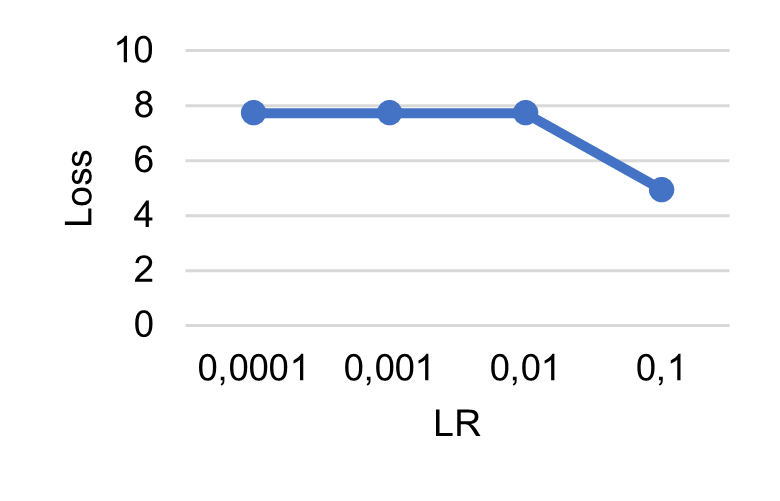
\includegraphics[width=5.0cm]{capitulos/metodos/imagens/otim_encdec_lstm_lr}
%         }%
%         % \hfill
%         \subcaptionbox{Dropout \label{subfig:otim-encdec-lstm-dropout}}{
%             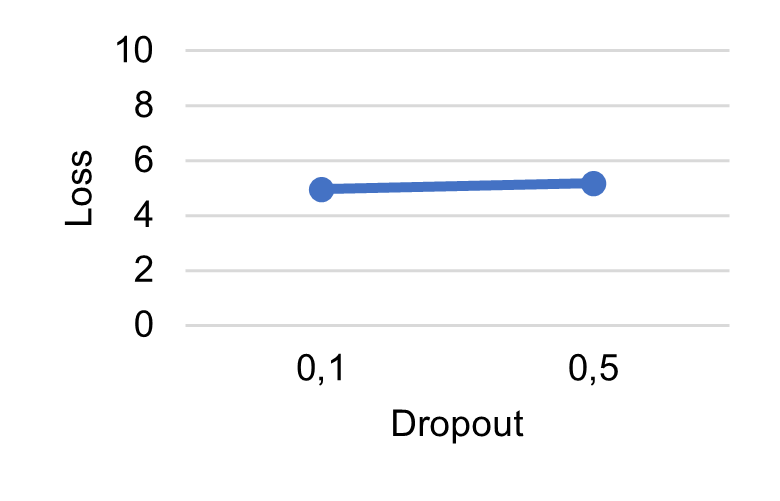
\includegraphics[width=5.0cm]{capitulos/metodos/imagens/otim_encdec_lstm_dropout}
%         }%
%         % \hfill
%         \subcaptionbox{Nº de camadas \label{subfig:otim-encdec-lstm-layers}}{
%             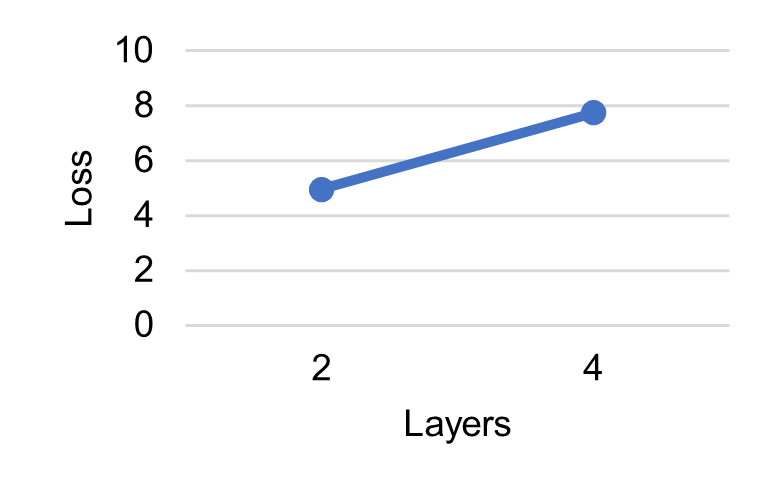
\includegraphics[width=5.0cm]{capitulos/metodos/imagens/otim_encdec_lstm_layers}
%         }%
%         \hfill
%         \subcaptionbox{Tamanho camadas ocultas \label{subfig:otim-encdec-lstm-hidden}}{
%             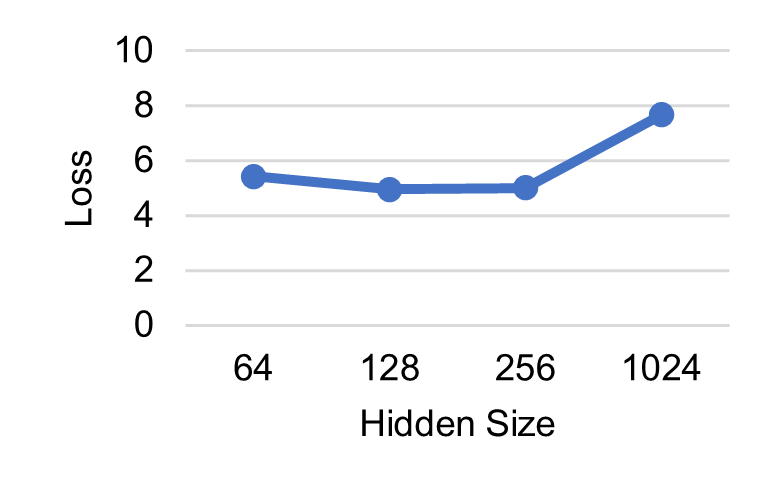
\includegraphics[width=5.0cm]{capitulos/metodos/imagens/otim_encdec_lstm_hidden_size}
%         }%
%         % \hfill
%         \subcaptionbox{Tamanho embeddings \label{subfig:otim-encdec-lstm-emb}}{
%             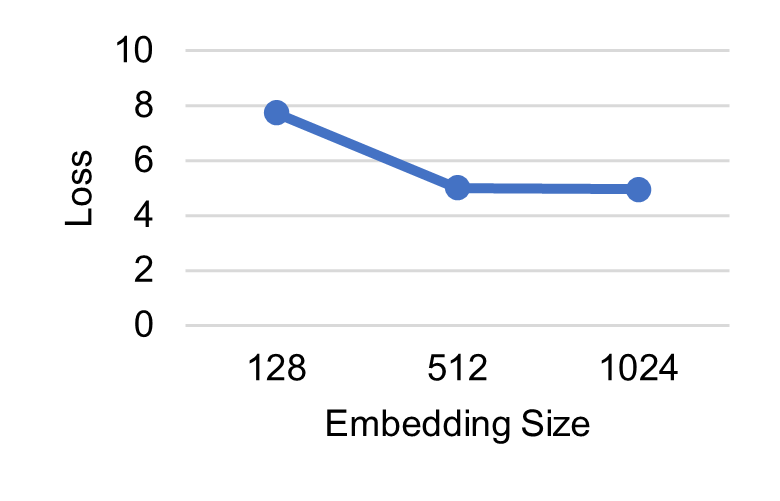
\includegraphics[width=5.0cm]{capitulos/metodos/imagens/otim_encdec_lstm_emb_size}
%         }%
%     }
%     \nomefonte{}
%     \label{fig:otim-encdec-lstm}
% \end{figure}

Para o \textit{Encoder-Decoder} com \acrshort{lstm} utilizamos o conjunto de parâmetros apresentados na \autoref{tab:otim-params-encdec} para essa busca e a configuração que melhor reduziu a perda do modelo foi a taxa de aprendizagem de 0,1; \textit{dropout} de 0,1; utilização de 2 camadas de \acrshort{lstm} no \textit{encoder} e no \textit{decoder}; camadas ocultas com dimensão de 128; e \textit{embeddings} com dimensão de 1024.
No caso do \textit{Encoder-Decoder} com \acrshort{gru} os parâmetros também são mostrados na \autoref{tab:otim-params-encdec} e a melhor combinação obtida foi a taxa de aprendizagem de 0,01; \textit{dropout} de 0,1; utilização de 2 camadas de \acrshort{gru} no \textit{encoder} e no \textit{decoder}; camadas ocultas com dimensão de 256; e \textit{embeddings} com dimensão de 512.

% Please add the following required packages to your document preamble:
% \usepackage{multirow}
% \usepackage{graphicx}
% \usepackage[table,xcdraw]{xcolor}
% If you use beamer only pass "xcolor=table" option, i.e. \documentclass[xcolor=table]{beamer}
\begin{table}[]
    \centering
    \caption{Parâmetros otimizados para o \textit{Encoder-Decoder} (\acrshort{lstm}) e o \textit{Encoder-Decoder} (\acrshort{gru}) com os respectivos valores calculados de perda}
    \label{tab:otim-params-encdec}
    \resizebox{0.8\textwidth}{!}{%
        \begin{tabular}{lr|rr}
            \hline
            \multicolumn{2}{l|}{\cellcolor[HTML]{EFEFEF}}                                                             & \multicolumn{2}{c}{\cellcolor[HTML]{EFEFEF}Perda}                                                                                                                                            \\ \cline{3-4}
            \multicolumn{2}{l|}{\multirow{-2}{*}{\cellcolor[HTML]{EFEFEF}Parâmetro}}                                  & \multicolumn{1}{c|}{\cellcolor[HTML]{EFEFEF}\textbf{Encoder-Decoder (LSTM)}} & \multicolumn{1}{c}{\cellcolor[HTML]{EFEFEF}\textbf{Encoder-Decoder (GRU)}}                                    \\ \hline
            \multicolumn{1}{l|}{}                                                                                     & 0,0001                                                                       & \multicolumn{1}{r|}{7,734553}                                              & 7,734372                         \\
            \multicolumn{1}{l|}{}                                                                                     & 0,001                                                                        & \multicolumn{1}{r|}{7,734348}                                              & 7,725883                         \\
            \multicolumn{1}{l|}{}                                                                                     & 0,01                                                                         & \multicolumn{1}{r|}{7,732680}                                              & \cellcolor[HTML]{FFF5E1}4,528818 \\
            \multicolumn{1}{l|}{\multirow{-4}{*}{Taxa de aprendizagem}}                                               & 0,1                                                                          & \multicolumn{1}{r|}{\cellcolor[HTML]{FFF5E1}4,945398}                      & 4,588312                         \\ \hline
            \multicolumn{1}{l|}{}                                                                                     & 0,1                                                                          & \multicolumn{1}{r|}{\cellcolor[HTML]{FFF5E1}4,945398}                      & \cellcolor[HTML]{FFF5E1}4,528818 \\
            \multicolumn{1}{l|}{\multirow{-2}{*}{Dropout}}                                                            & 0,5                                                                          & \multicolumn{1}{r|}{5,165860}                                              & 4,726675                         \\ \hline
            \multicolumn{1}{l|}{}                                                                                     & 128                                                                          & \multicolumn{1}{r|}{7,733999}                                              & 5,375009                         \\
            \multicolumn{1}{l|}{}                                                                                     & 512                                                                          & \multicolumn{1}{r|}{4,999395}                                              & \cellcolor[HTML]{FFF5E1}4,528818 \\
            \multicolumn{1}{l|}{\multirow{-3}{*}{Tamanho embeddings}}                                                 & 1024                                                                         & \multicolumn{1}{r|}{\cellcolor[HTML]{FFF5E1}4,945398}                      & 4,544811                         \\ \hline
            \multicolumn{1}{l|}{}                                                                                     & 64                                                                           & \multicolumn{1}{r|}{5,416092}                                              & 5,017869                         \\
            \multicolumn{1}{l|}{}                                                                                     & 128                                                                          & \multicolumn{1}{r|}{\cellcolor[HTML]{FFF5E1}4,945398}                      & 4,544811                         \\
            \multicolumn{1}{l|}{}                                                                                     & 256                                                                          & \multicolumn{1}{r|}{4,999395}                                              & \cellcolor[HTML]{FFF5E1}4,528818 \\
            \multicolumn{1}{l|}{\multirow{-4}{*}{\begin{tabular}[c]{@{}l@{}}Tamanho camadas \\ ocultas\end{tabular}}} & 1024                                                                         & \multicolumn{1}{r|}{7,662058}                                              & 4,920857                         \\ \hline
            \multicolumn{1}{l|}{}                                                                                     & 2                                                                            & \multicolumn{1}{r|}{\cellcolor[HTML]{FFF5E1}4,945398}                      & \cellcolor[HTML]{FFF5E1}4,528818 \\
            \multicolumn{1}{l|}{\multirow{-2}{*}{Nº de camadas}}                                                      & 4                                                                            & \multicolumn{1}{r|}{7,734541}                                              & 5,915603                         \\ \hline
        \end{tabular}%
    }
    \nomefonte{}
\end{table}


% % Parâmetros otimizados para Encoder-Decoder (GRU):
% \begin{figure}[ht!]
%     \centering
%     \caption{\textmd{Parâmetros otimizados para o \textit{Encoder-Decoder} com \acrshort{gru}}}
%     \borda[\textwidth]{
%         \subcaptionbox{Taxa de aprendizagem \label{subfig:otim-encdec-gru-lr}}{
%             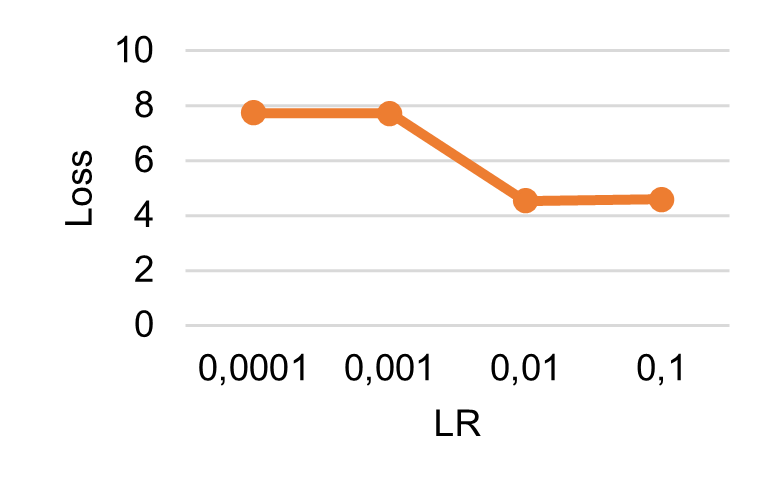
\includegraphics[width=5.0cm]{capitulos/metodos/imagens/otim_encdec_gru_lr}
%         }%
%         % \hfill
%         \subcaptionbox{Dropout \label{subfig:otim-encdec-gru-dropout}}{
%             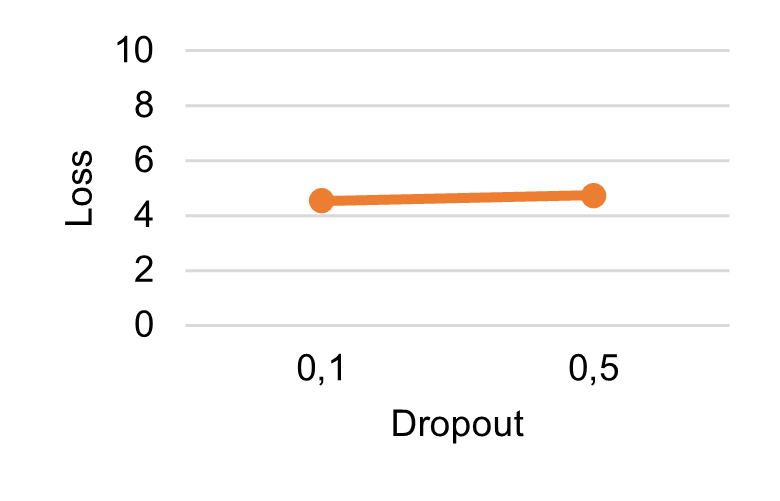
\includegraphics[width=5.0cm]{capitulos/metodos/imagens/otim_encdec_gru_dropout}
%         }%
%         % \hfill
%         \subcaptionbox{Nº de camadas \label{subfig:otim-encdec-gru-layers}}{
%             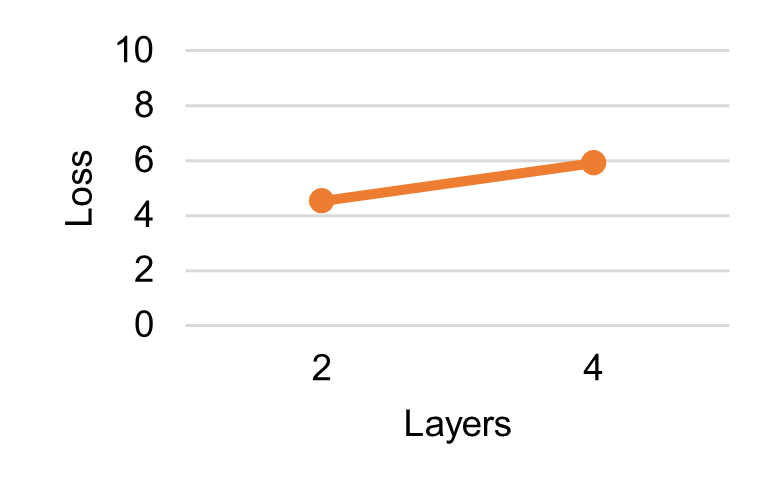
\includegraphics[width=5.0cm]{capitulos/metodos/imagens/otim_encdec_gru_layers}
%         }%
%         \hfill
%         \subcaptionbox{Tamanho camadas ocultas\label{subfig:otim-encdec-gru-hidden}}{
%             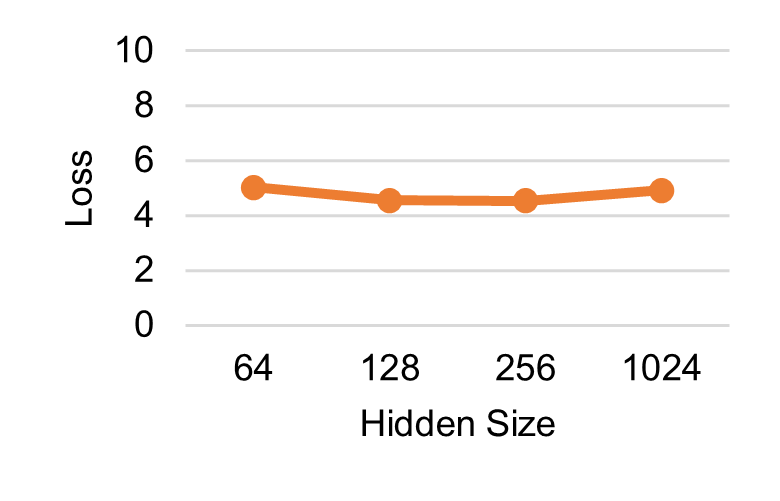
\includegraphics[width=5.0cm]{capitulos/metodos/imagens/otim_encdec_gru_hidden_size}
%         }%
%         % \hfill
%         \subcaptionbox{Tamanho embeddings\label{subfig:otim-encdec-gru-emb}}{
%             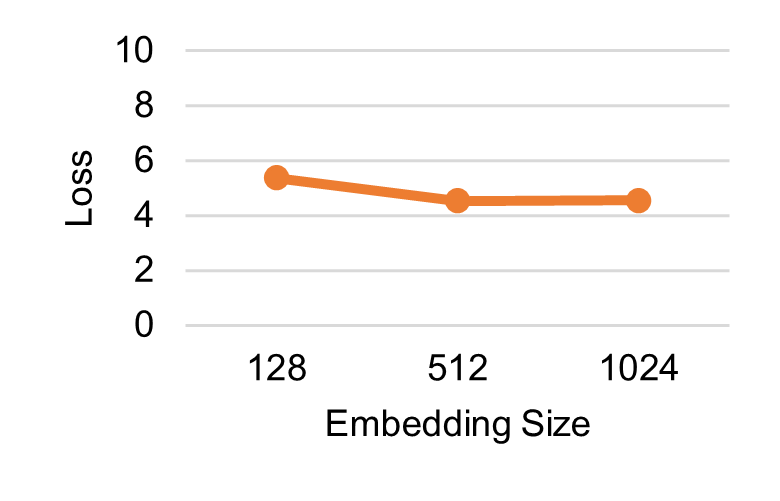
\includegraphics[width=5.0cm]{capitulos/metodos/imagens/otim_encdec_gru_emb_size}
%         }%
%     }
%     \nomefonte{}
%     \label{fig:otim-encdec-gru}
% \end{figure}



% % Parâmetros otimizados para Transformer:
% \begin{figure}[ht!]
%     \centering
%     \caption{\textmd{Parâmetros otimizados para o \textit{Transformer}}}
%     \borda[\textwidth]{
%         \subcaptionbox{Taxa de aprendizagem \label{subfig:otim-transformer-lr}}{
%             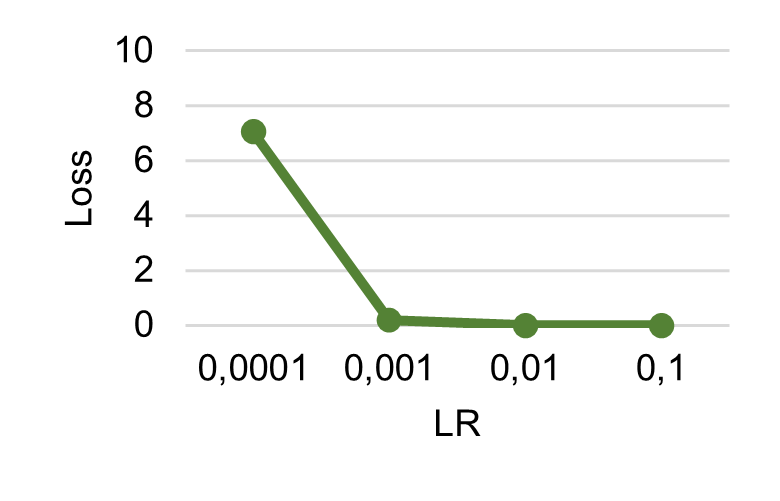
\includegraphics[width=5.0cm]{capitulos/metodos/imagens/otim_transformer_lr}
%         }%
%         % \hfill
%         \subcaptionbox{Dropout \label{subfig:otim-transformer-dropout}}{
%             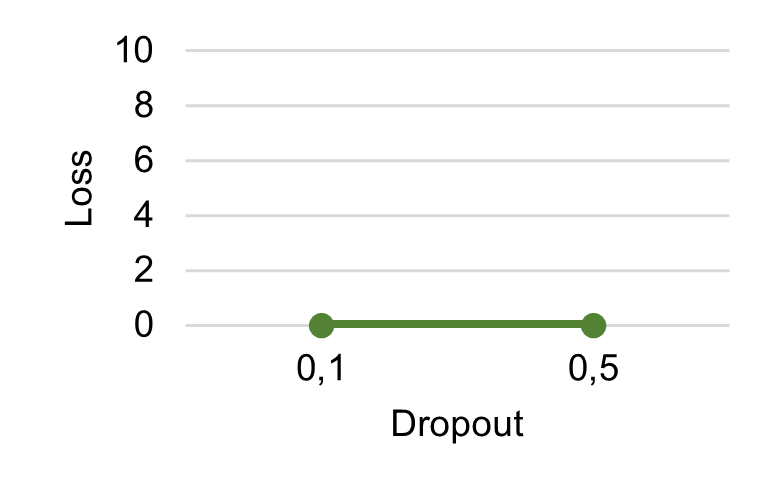
\includegraphics[width=5.0cm]{capitulos/metodos/imagens/otim_transformer_dropout}
%         }%
%         % \hfill
%         \subcaptionbox{Nº de camadas \label{subfig:otim-transformer-layers}}{
%             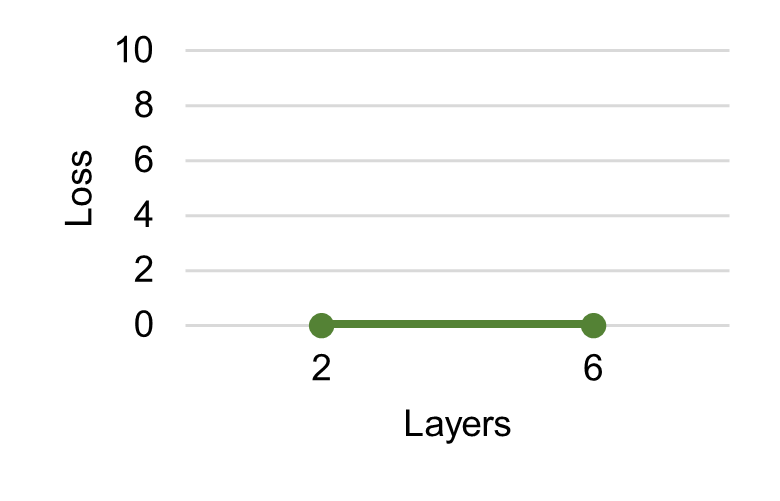
\includegraphics[width=5.0cm]{capitulos/metodos/imagens/otim_transformer_layers}
%         }%
%         \hfill
%         \subcaptionbox{Tamanho camadas ocultas\label{subfig:otim-transformer-hidden}}{
%             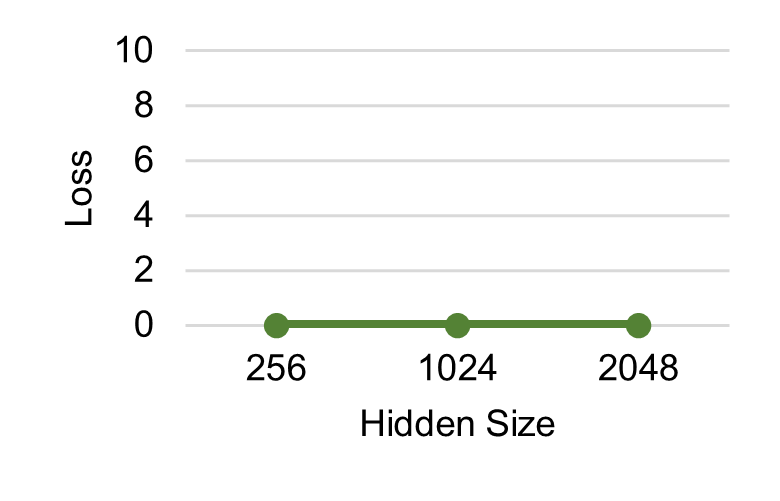
\includegraphics[width=5.0cm]{capitulos/metodos/imagens/otim_transformer_hidden_size}
%         }%
%         % \hfill
%         \subcaptionbox{Tamanho embeddings\label{subfig:otim-transformer-emb}}{
%             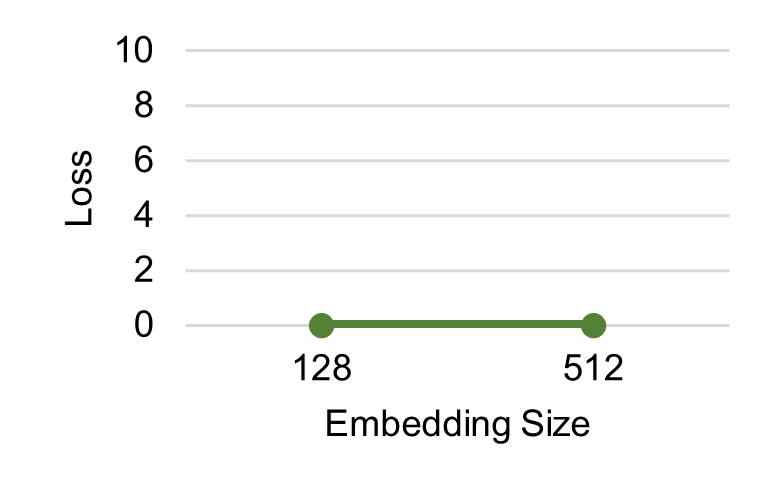
\includegraphics[width=5.0cm]{capitulos/metodos/imagens/otim_transformer_emb_size}
%         }%
%         % \hfill
%         \subcaptionbox{Nº de cabeças\label{subfig:otim-transformer-heads}}{
%             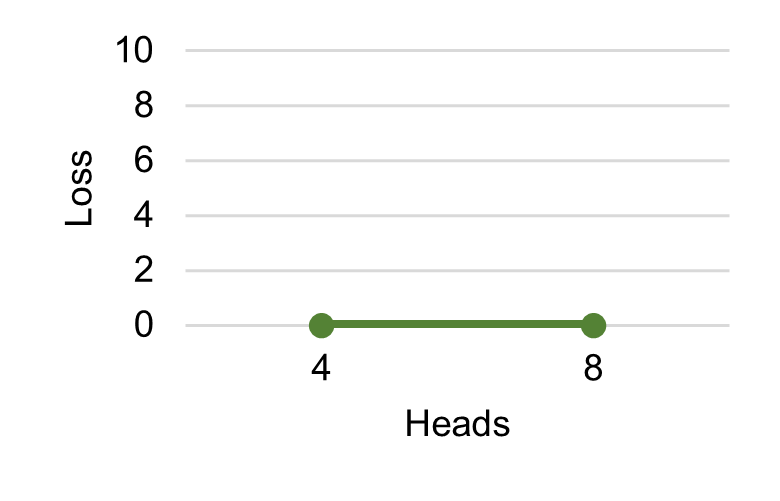
\includegraphics[width=5.0cm]{capitulos/metodos/imagens/otim_transformer_heads}
%         }%
%     }
%     \nomefonte{}
%     \label{fig:otim-transformer}
% \end{figure}


% Please add the following required packages to your document preamble:
% \usepackage{multirow}
% \usepackage{graphicx}
% \usepackage[table,xcdraw]{xcolor}
% If you use beamer only pass "xcolor=table" option, i.e. \documentclass[xcolor=table]{beamer}
\begin{table}[]
    \centering
    \caption{Parâmetros otimizados para o \textit{Transformer} com os respectivos valores calculados de perda}
    \label{tab:otim-params-transf}
    \resizebox{0.42\textwidth}{!}{%
        \begin{tabular}{lr|r}
            \hline
            \rowcolor[HTML]{EFEFEF}
            \multicolumn{2}{l|}{\cellcolor[HTML]{EFEFEF}}                                                             & \multicolumn{1}{c}{\cellcolor[HTML]{EFEFEF}Perda}                                                   \\ \cline{3-3}
            \rowcolor[HTML]{EFEFEF}
            \multicolumn{2}{l|}{\multirow{-2}{*}{\cellcolor[HTML]{EFEFEF}Parâmetro}}                                  & \multicolumn{1}{c}{\cellcolor[HTML]{EFEFEF}\textbf{Transformer}}                                    \\ \hline
            \multicolumn{1}{l|}{}                                                                                     & 0,0001                                                           & 7,052482                         \\
            \multicolumn{1}{l|}{}                                                                                     & 0,001                                                            & 0,184165                         \\
            \multicolumn{1}{l|}{}                                                                                     & 0,01                                                             & 0,000000                         \\
            \multicolumn{1}{l|}{\multirow{-4}{*}{Taxa de aprendizagem}}                                               & 0,1                                                              & \cellcolor[HTML]{FFF5E1}0,000000 \\ \hline
            \multicolumn{1}{l|}{}                                                                                     & 0,1                                                              & 0,000001                         \\
            \multicolumn{1}{l|}{\multirow{-2}{*}{Dropout}}                                                            & 0,5                                                              & \cellcolor[HTML]{FFF5E1}0,000000 \\ \hline
            \multicolumn{1}{l|}{}                                                                                     & 128                                                              & \cellcolor[HTML]{FFF5E1}0,000000 \\
            \multicolumn{1}{l|}{\multirow{-2}{*}{Tamanho embeddings}}                                                 & 512                                                              & 0,000000                         \\ \hline
            \multicolumn{1}{l|}{}                                                                                     & 256                                                              & \cellcolor[HTML]{FFF5E1}0,000000 \\
            \multicolumn{1}{l|}{}                                                                                     & 1024                                                             & 0,000000                         \\
            \multicolumn{1}{l|}{\multirow{-3}{*}{\begin{tabular}[c]{@{}l@{}}Tamanho camadas \\ ocultas\end{tabular}}} & 2048                                                             & 0,000000                         \\ \hline
            \multicolumn{1}{l|}{}                                                                                     & 2                                                                & \cellcolor[HTML]{FFF5E1}0,000000 \\
            \multicolumn{1}{l|}{\multirow{-2}{*}{Nº de camadas}}                                                      & 6                                                                & 0,000001                         \\ \hline
            \multicolumn{1}{l|}{}                                                                                     & 4                                                                & \cellcolor[HTML]{FFF5E1}0,000000 \\
            \multicolumn{1}{l|}{\multirow{-2}{*}{Nº de cabeças}}                                                      & 8                                                                & 0,000000                         \\ \hline
        \end{tabular}%
    }
    \nomefonte{}
\end{table}


Por fim, para o \textit{Transformer} utilizamos os parâmetros mostrados na \autoref{tab:otim-params-transf}. A melhor combinação obtida foi a taxa de aprendizagem de 0,1; \textit{dropout} de 0,5; utilização de 2 camadas; camadas ocultas com dimensão de 256; \textit{embeddings} com dimensão de 128; e utilização de 2 cabeças de \textit{attention}.


O código-fonte utilizado nos experimentos deste trabalho foi disponibilizado através do endereço indicado abaixo\footnote{
    Disponível em \url{https://www.cin.ufpe.br/~cca5/sl-nlp}.
}.



% \cite{goodfellow-2016-deep-learning}

% --------
% A reasonable choice of optimization algorithm is SGD with momentum with a decaying learning rate (popular decay schemes that perform better or worse on different problems include decaying linearly until reaching a fixed minimum learning rate, decaying exponentially, or decreasing the learning rate by a factor of 2–10 each time validation error plateaus).

% - optimizer: SGD
%     nesterov: False
%     momentum: 0.9
% --------
% Loss function

% - criterion: CrossEntropyLoss

% --------
% Early stopping should be used almost universally.

% - training_args:
%     max_epochs: 50
%     batch_size: 50
%     lr: 0.01
%     test_size: 0.15
%     valid_size: 0.15
%     early_stopping:
%         patience: 10
%         threshold: 10e-4
%         threshold_mode: rel
%     gradient_clipping:
%         gradient_clip_value: 0.5
%     lr_scheduler: 
%         policy: ReduceLROnPlateau
%         factor: 0.2
%         patience: 5

% --------
% Learning rate - apresentar graficos?
% - learning rate (grid search)


% --------
% - dimensões dos modelos

%     Transformer (selecionamos as dimensões do modelo clássico \cite{vaswani-2017-transformer})
%         embedding_size: 512
%         hidden_size: 2048
%         num_layers: 6
%         dropout: 0.1
%         num_heads: 8

